\section {Sulfur Dioxide Bonding Coordinations}

To further assess the effect of temperature on \suldiox~behavior we turn to analysis of the bonds formed between \suldiox~and the water surface. The bonding coordinations were determined for the \suldiox~based on the bondlength criteria noted in the introduction. Bonds formed between \suldiox-sulfur and \wat-oxygen are labeled 'S' coordinated, and bonds formed between \suldiox-oxygen and \wat-hydrogen are labeled 'O' coordinated. For each bond an additional letter label is appended to the coordination. For example, an 'SOO' coordinated \suldiox~forms three bonds to waters: two bonds are formed through the \suldiox-oxygens, and one through the \suldiox~sulfur. This naming scheme is taken from the work of Baer et al. where the \suldiox~bonding distribution was determined for a surface molecule at a single temperature simulated under similar conditions.\cite{Baer2010}

Figure \ref{fig:so2-bonding-coordinations} shows the distribution of bonding coordinations throughout the set of simulated trajectories for both the cold and hot temperatures.

% Figure showing all the different types of so2 coordinations
\begin{figure}[h!]
	\begin{center}
		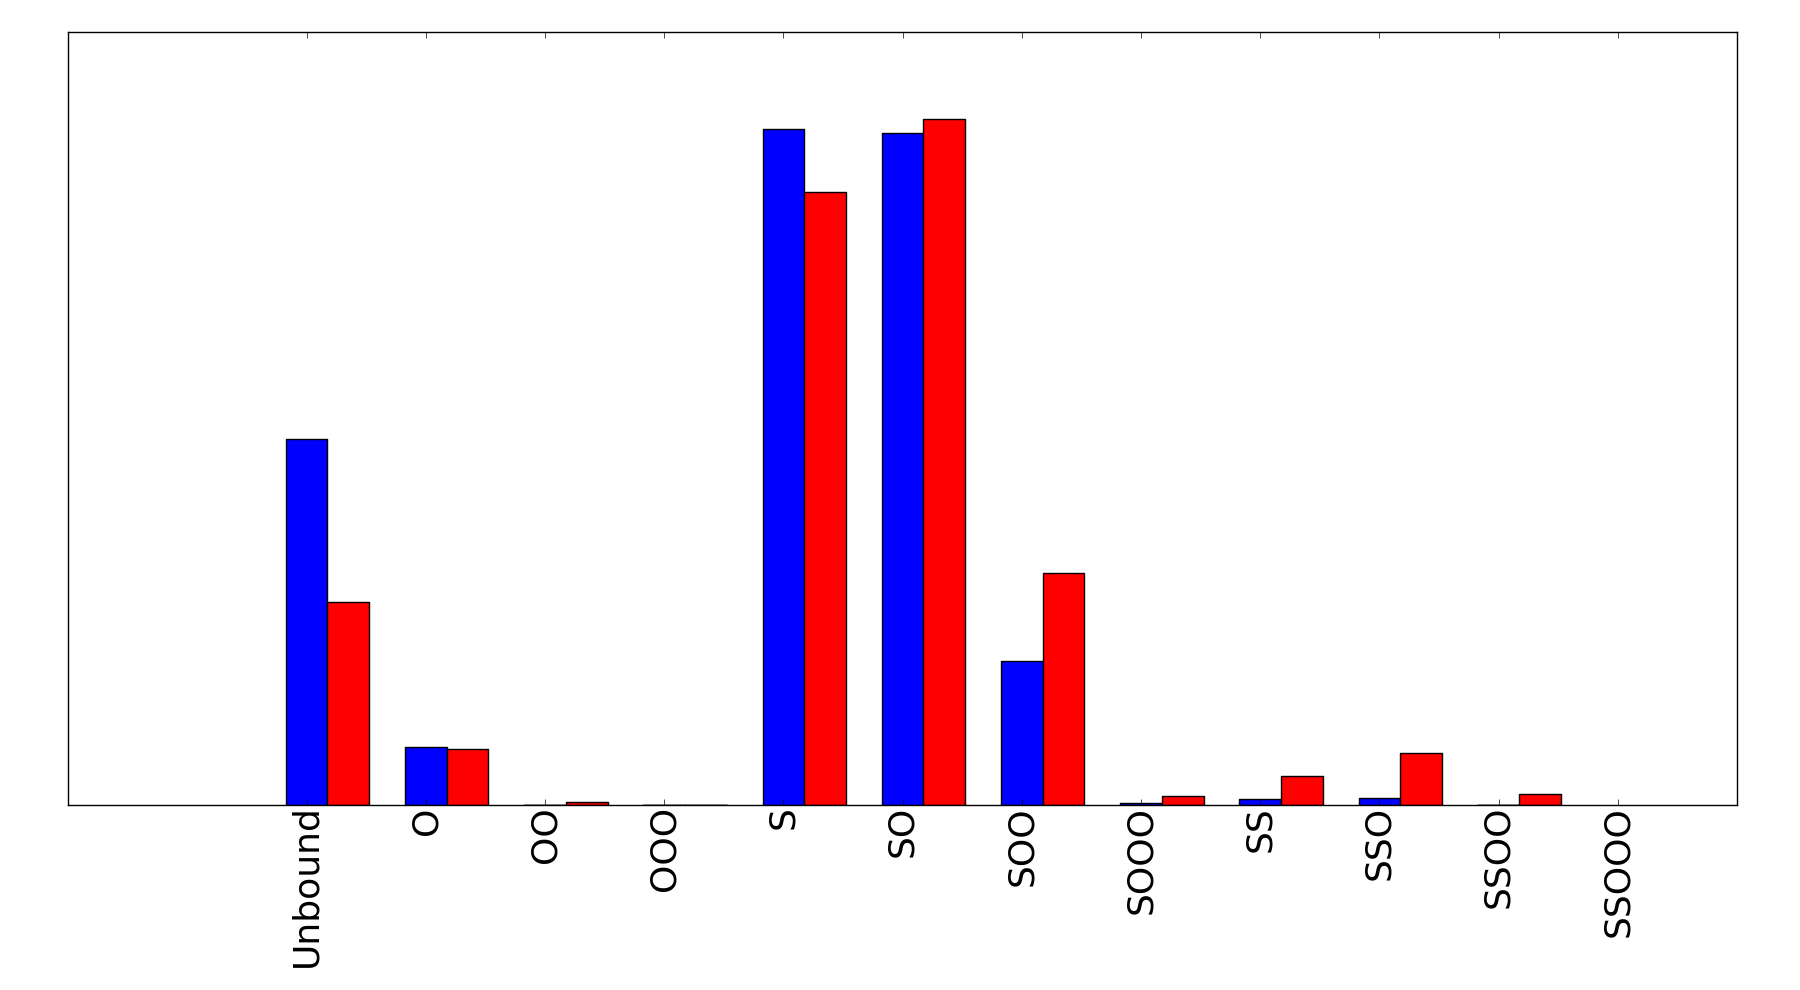
\includegraphics[scale=1.0]{images/coordination/so2-bonding-coordinations.png}
		\caption{}
		\label{fig:so2-bonding-coordinations}
	\end{center}
\end{figure}


\begin{figure}[h!]
	\begin{center}
		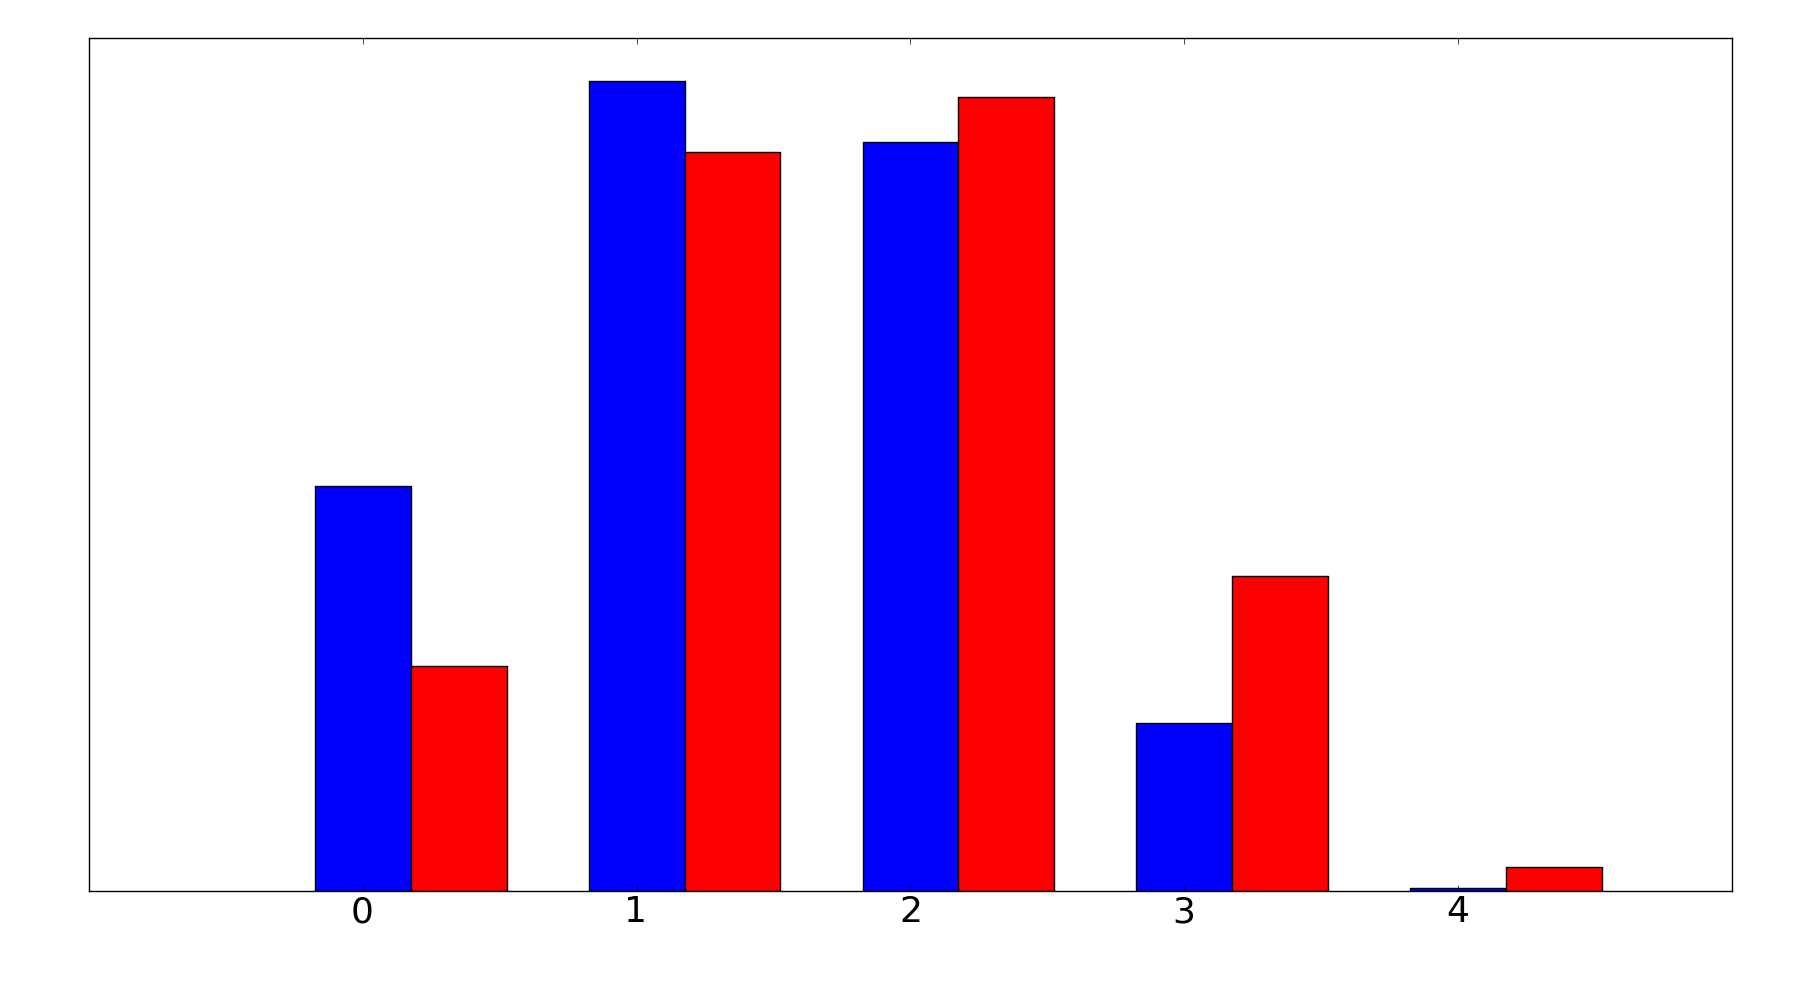
\includegraphics[scale=1.0]{images/coordination/so2-Total-number-bonds.png}
		\caption{}
		\label{fig:so2-bonding-coordinations}
	\end{center}
\end{figure}

\begin{figure}[h!]
	\begin{center}
		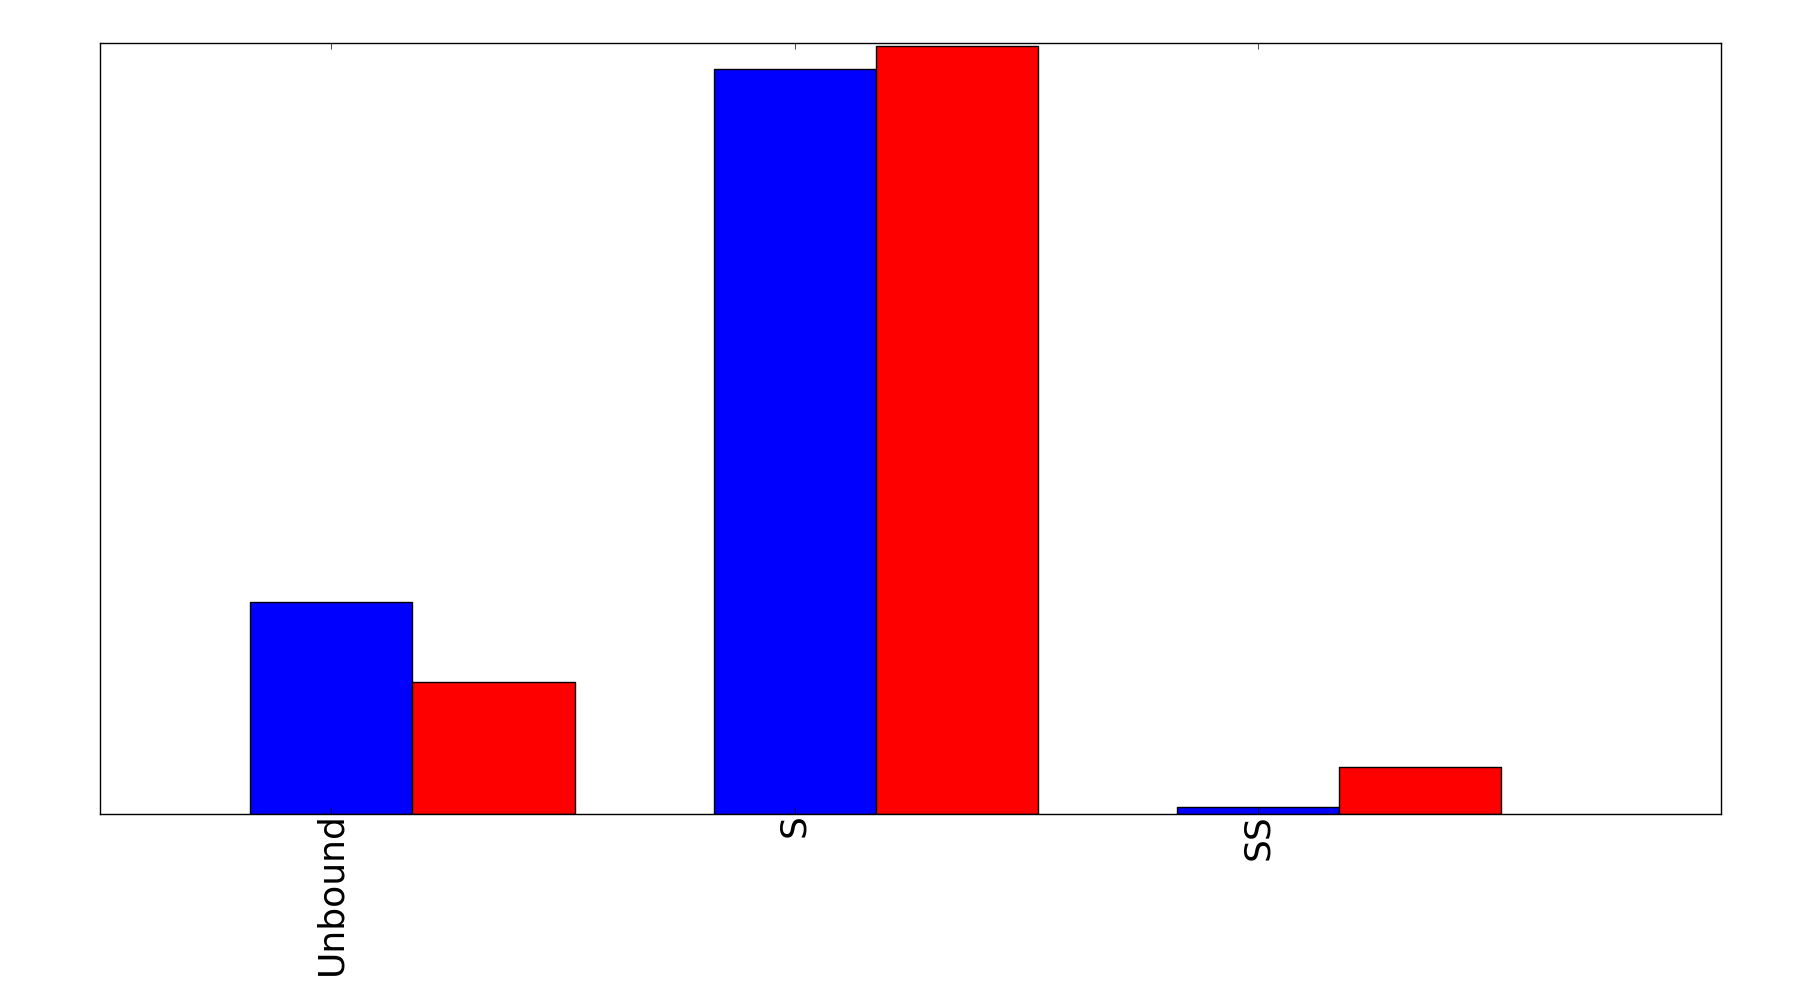
\includegraphics[scale=1.0]{images/coordination/so2-S-bonding-coordinations.png}
		\caption{}
		\label{fig:so2-bonding-coordinations}
	\end{center}
\end{figure}

\begin{figure}[h!]
	\begin{center}
		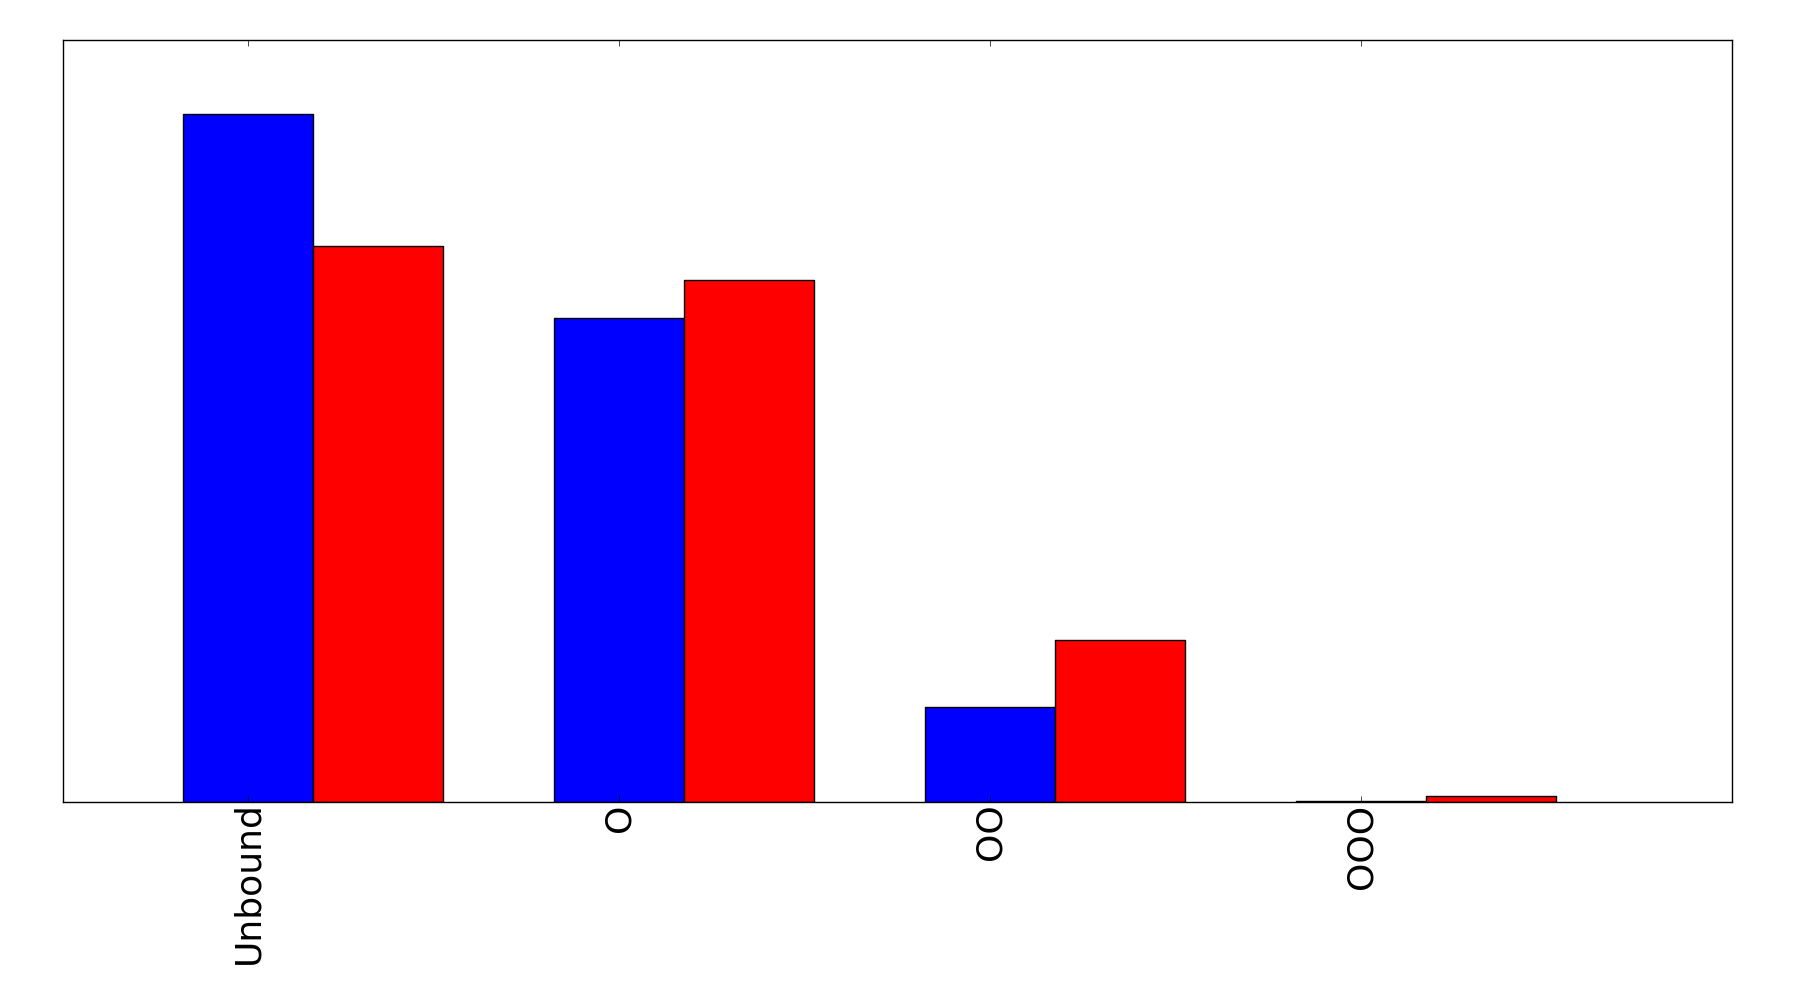
\includegraphics[scale=1.0]{images/coordination/so2-O-bonding-coordinations.png}
		\caption{}
		\label{fig:so2-bonding-coordinations}
	\end{center}
\end{figure}
